% !TeX spellcheck = en_US
\documentclass{sig-alternate}

\usepackage[ampersand]{easylist}
\usepackage{amsmath}

\usepackage{algpseudocode} 
\usepackage{algorithm}

\usepackage{graphicx}

\usepackage{url}
%\usepackage{hyperref}

\usepackage{etoolbox}
\makeatletter
\def\@copyrightspace{\relax}
\makeatother

\newcommand{\mli}[1]{\mathit{#1}}

%\declareGraphicsExtensions{.pdf,.png,.jpg}

%\numberwithin{equation}{subsection}

\begin{document}

\title{Project report}

\subtitle{IN4336 Combinatorial Algorithms\\Project 3: Graph Coloring: applications, approximations and
solvers}

\numberofauthors{2}

\author{
\alignauthor
David Hoepelman\\
       \affaddr{1521969}\\
\alignauthor
Luis Garcia Rosario\\
       \affaddr{4062949}
}

\maketitle

%\begin{abstract}
%content...
%end{abstract}

\begin{abstract}

\end{abstract}

% Lingeling was chosen because it performed well in a large number of categories in the recent SAT Competition 2014 (http://www.satcompetition.org/2014/) contest

\section{Introduction}

Solvers for NP-Hard problems can be used to solve instances of other NP-Hard problems by polynomially transforming the other problem instance. This is called an encoding.
This possibility makes it feasible to make highly-optimized solving algorithms called solvers for certain relatively general NP-Hard problems.

For most popular problems multiple solvers exists, and benchmarks are available or contests are held to compare them.
However comparisons between problems are rarer and in this project we will do such a comparison.
We want to see if some problems are more suitable to encode other problems in or if the choice of problem to encode to makes little impact.

Another question is whether translations into intermediary problems add significant overhead.
While we know that polynomial transformations do not increase the complexity of a NP-Hard problem, it might still have a practical impact in how fast a problem instance can be solved or what the largest solvable problem instance is.
With this we want to see if encodings can be viably done in smaller easier steps, or if it is better to encode the problem directly into the target problem.

We formulated the following research question for this project:

\begin{enumerate}
\item[RQ1]{Is there a speed difference between different target problems when solving an identical translated problem instance?}
\item[RQ2]{Are intermediate transformations viable?}
	\begin{enumerate}
	\item[RQ2.1]{Does an intermediate transformation significantly decrease the speed with which problem instances can be solved?}
	\item[RQ2.2]{Does an intermediate transformation decrease the size of the largest possible problem instances which can be solved?}
	\end{enumerate}
\end{enumerate}

In answering our research questions we will focus on solvers for \emph{Integer Linear Programming} (ILP), \emph{Satisfiability} (SAT) and \emph{Satisfiability Modulo Theories} (SMT).

As problems to encode we will focus on the \emph{Resource Constrained Project Scheduling Problem} (RCPSP) and \emph{Graph Coloring} (GC).

\section {Target problems}

\subsubsection*{Satisfiability (SAT)}

The satisfiability problem is informally defined as given a boolean formula in conjunctive normal form (CNF), find an assignment that makes the formula true.
A formula is in CNF if it is a conjunction of clauses ($C_1 \wedge C_2 \wedge \ldots \wedge C_n$) where each clause is a disjunction of literals ($l_1 \lor l_2 \lor \ldots \lor l_n$) where each literal is a variable or the negation of a variable ($p$ or $\neg p$).
All propositional formulas can be converted to CNF.
A SAT solver will find either a valid assignment for the given formula, or will report that it is unsatisfiable.

\subsubsection*{Satisfiability Modulo Theories (SMT)}

Satisfiability Modulo Theories is a generalization of satisfiability.
A SMT problem instance is still a given formula, and the problem is to find out if it is satisfiable.
However, a variable can now be a predicate, a function which evaluates to a boolean, over non-boolean variables and operators.
Commonly SMT solvers support integer, real, integer array and bitvector variables and linear or non-linear arithmatic, but other extensions are possible.

The concrete advantage of this is that certain constraints which are hard to specifiy in a pure boolean formula can now be specified in a more natural language.

\subsubsection*{Integer Linear Programming (ILP)}

An Integer Linear Program is a linear program (LP) that has the additional contraint that all variables must be integers. 
An ILP problem is an optimization problem where the objective is to maximize or minimize some value. 
The encoding of an optimization problem into ILP starts by composing an objective function in order to find the optimal objective value.
Then, the objective function is subjected to one or more constraints functions. Each function listed representing a different constraint.
The variables used in these functions may be bounded, e.g. in 0-1 ILP encoding variables can take a value of 0 or 1.
Finally, the last constraint in ILP is the integrallity constraint, meaning that all variables must take integers.

\section{Solving optimization problems with decidability solvers}
\label{sec:OptWithDec}

A decidability solver finds a feasible solution to a problem instance.
In practice one does often not only which to find \emph{a} feasible solution, but one wants to find \emph{the best} feasible solution out of all feasible solutions.
This is called an optimization problem.

ILP is an optimization problem and can thus naturally be used as a target for optimization problems.
To use decidability solvers for an optimization problem one can formulate the optimization problem as a sequence of decision problems $P$ with cost $c \in \mathbb{N}$.
In each step the solver looks for a solution to $P_c$.

We independently though of two ways to go through this sequence, but they are identical too the approaches described by Wille et. Al \cite{wille2008using}.
We will use their terminology.

The first approach called the \emph{iterative approach} starts at the lower bound of the possible costs $c = \mli{LB}$, usually $\mli{LB} = 0$.
While the solver can find no solution for $P_c$, $c$ is incremented.
In pseudocode:

\begin{algorithmic}
\State $c \gets \mli{UB}$
\While {not $solvable$}
	\State $P \gets encode(instance, c)$
	\State $solvable \gets solve(P)$
	\If {not $solvable$}
		\State $c++$
	\EndIf
\EndWhile
\State $\mli{OPT} \gets c$
\end{algorithmic}

This approach has the obvious disadvantage that $\mli{OPT}-\mli{LB}$ iterations are needed which is especially problematic if $\mli{OPT}$ is large

An alternative approach is too determine increasingly better lower and upper bounds.
If $P_c$ is determined feasible, one can look for a solution to $P_{c'}$ with $c' < c$. Likewise if $P_c$ is unfeasible, one can look for a solution to $P_{c'}$ with $c' > c$.
The minimal cost $OPT$ is found when $P_{OPT-1}$ is unfeasible, and $P_{\mli{OPT}}$ is feasible. This is called to approximation approach.
In pseudocode:

\begin{algorithmic}
\While {$\mli{LB} \neq \mli{UB} - 1$}
	\State $c = \mli{LB} + \lceil \frac{\mli{UB} - \mli{LB}}{2} \rceil$
	\State $P \gets encode(instance, c)$
	\State $solvable \gets solve(P)$
	\If {$solvable$}
		\State $\mli{UB} \gets c$
	\Else
		\State $\mli{LB} \gets c$
	\EndIf
\EndWhile
\State $\mli{OPT} \gets \mli{UB}$
\end{algorithmic}

By performing a binary search over all possible $c$, we set the maximum number of iterations to $\lceil log_2(\mli{UB}-\mli{LB}) \rceil$.

During our experiments we encountered the problem that the first problem $P_{\frac{1}{2}\mli{UB}}$ took a long time to encode, even though it usually was satisfiable.
To get around this better upper bounds were needed, for which we tested both theoretical upper bounds and approximation algorithms.


\section{Graph Coloring}
\label{sec:graph_coloring}

The graph coloring problem is one of the Karp's 21 original NP-Complete problems \cite{karp1972reducibility}.
Graph coloring exists in several variants, but they are all reducible to the vertex coloring problem.
We chose the optimization variant of the vertex coloring problem which is informally defined as given an undirected graph $G = (V,E)$, find the minimal number of colors $k$ needed to color each vertex so that no adjacent vertex shares a color.
More formally:
\begin{subequations}
\begin{align*}
        & G = (V,E) & E \subseteq V^2\\
        & map : V \rightarrow [1,k] & k \in \mathbb{N} \\
        & \text{with } map(v) \neq map(w) & (v,w) \in E \\
        & VC = min\{k \ | \  map : V \rightarrow [1,k]\}
\end{align*}
\end{subequations}

\subsection{Bounds}

The possible values of $k$ have clearly defined bounds.
All graphs except the empty graph will need at least $1$ color, and all graphs with an edge will need at least $2$ colors.
We stuck with an lower bound of $0$ for the approximation approach and $1$ for the iteration approach.

The trivial upper bound for a graph is $|V|$ colors, as every vertex can have its own unique color in that case.
Another useful upper bound is $max(degree(v))+1 \text{ for } v \in V$, the degree being the number of neighbors or edges of a node.
This u

\subsection{SAT encoding}

As satisfiability is a decision problem $k$ needs to be a parameter of the transformation, see section \ref{sec:OptWithDec} for how we determined $k$.

We adopted the encoding from \cite{cs395tGCtoSAT}.
We define a variable for every node and color combination $p_{vi} (v \in V, i \in [1,k])$.
If node $v$ has color $i$ then $p_{vi}$, otherwise $\neg p_{vi}$.
The following clauses ensure that the assignment will be valid for the GC instance:

\setcounter{equation}{1}
\begin{subequations}
\begin{align}
        & \bigvee_{1 \leq i \leq k} p_{vi}& v \in V\\
        & \neg p_{vi} \lor \neg p_{vj} & v \in V, 1 \leq i < j \leq k \\
        & \neg p_{vi} \lor \neg p_{wi} & v \in V, 1 \leq i \leq k
\end{align}
\end{subequations}

Clauses of type 2a ensures that every node has one or more colors. Clauses of type 2b ensures every node has at most one color. Clauses of type 2c ensure that nodes that share an edge do not have the same color.
The encoding uses $O(|V| k)$ variables and $O(|E|+|V| \cdot k^2)$ clauses.

There is another possible encoding which uses $O(|V| \cdot \lceil{log_2{k}\rceil})$ variables and $O(2^{\lceil{log_2k}\rceil} \cdot |E|+(2^{\lceil{log_2k\rceil}}-k) \cdot |V|)$ clauses which shows promising results in \cite{wille2008using}.
Unfortunately we did not have time to implement and test this encoding, we refer to section \ref{relatedandfuture}.

\subsection{SMT encoding}
Our SMT encoding is identical to our SAT encoding.
There are several candidate encodings which do use this additional expressive power, which are detailed in the future work section.

\subsection{ILP encoding}
The combinatorial problem of graph coloring can also be formulated as an 0-1 ILP in which the variables are binary variables. 
An advantage of using ILP is that unlike SAT and SMT, it can solve optimization problems. 
The 0-1 ILP formulation of the graph coloring problem,
can be done by taking the set of nodes V = {1,...,\emph{n}} of the graph G and the number of 
colors is $1 \leq \emph{k} \leq |V|$. By observing that a graph cannot use more colors than it's maximum 
degree, we put the upper bound for color \emph{k} as the highest degree of G.
Then, each color is represented by a binary variable \emph{$y_k$}, 
with \emph{k} = 1,...,\emph{n}, that indicatates whether color \emph{k} is used (\emph{$y_k$} = 1) or 
not (\emph{$y_k$} = 0). An objective function is formed by adding up these variables 
($\sum\limits_{k=1}^n \emph{$y_k$}$) to obtain the minimum sum. That is, we want the minimum number 
of the variables \emph{$y_k$} that are equal to 1. Furthermore, a binary variable \emph{$x_{ik}$} is 
used for each node-color combination to indicate whether node \emph{i} has received a color \emph{k} 
(\emph{$x_{ik}$} = 1) or not (\emph{$x_{ik}$} = 0). In the resulting 0-1 ILP in formal description 
listed below, adopted from \cite{faigle2002mathprogramming}, contraint (1) guarantees that each node 
is colored, (2) node \emph{i} receives color \emph{k} only if color \emph{k} has been used, (3) adjecent nodes should have different colors:
\begin{subequations}
\begin{align*}
        & & & min \sum\limits_{k=1}^n \emph{$y_k$} & & \\
        &  (1) & & \sum\limits_{k=1}^n \emph{$x_{ik}$} = 1 & & \emph{i} = 1,...,\emph{n} \\
        &  (2) & & \emph{$x_{ik}$} - \emph{$y_k$} \leq 0 & & \emph{i,k} = 1,...,\emph{n} \\
        &  (3) & &  \emph{$x_{ik}$} + \emph{$x_{jk}$} \leq 1 & & (i,j) \in E, \emph{k} = 1,...,\emph{n} \\
        &  (4) & & 0 \leq \emph{$x_{ik}$}, \emph{$y_k$} \leq 1 & & \\
        &  (5) & & \emph{$x_{ik}$}, \emph{$y_k$} \in \mathbb{Z} & &
\end{align*}
\end{subequations}

\section{RCPSP}
\label{sec:RCPSP}
The Resource Constraint Project Scheduling Problem (RCPSP) is informally defined as given a project with resource limits, jobs with dependencies and resource consumption of jobs, find an optimal schedule so that at no time too much resources are consumed and the project is completed at the earliest time possible.

\subsection{Formal definition and notation}
Given a project $P$ with:
\begin{itemize}
\item A set of jobs $V = \{1,\ldots,N\}$ 
\item A set of resources $\mathcal{R} = \{1,\ldots,M\}$
\item Precedence relations $(i,j) \in E \subset V \times V$ in which $(i,j)$ means job $j$ is dependent upon job $i$
\item Durations $d_i \in \mathbb{N}$ for each job $i \in V$
\item Resource limits $R_j$ for each $j \in \mathcal{R}$
\item Job resource consumptions $r_i,j$ for each job $i \in V$ and resource $j \in \mathcal{R}$
\end{itemize}

Define:
\begin{itemize}
\item The start time $s_i \in \mathbb{N}$ of job $i$ in the schedule
\item The finish time $f_i = s_i + d_i$ of job $i$
\item The in-progress status $u_{i,t} \in \{0,1\}$ of job $i$ at time $t$ in the schedule
\end{itemize}

Find the minimal make-span $T = \max_{i \in V}\{f_i\}$ subject to:
\begin{itemize}
\item Dependencies: \\ $f_i \leq s_j$ for every $(i,j) \in prec$
\item Resource constraints: \\ $\sum_{i \in V}{u_{i,t} \cdot r_{i,j}} \leq R_j$ for every $j \in R, t \in [0,T]$
\end{itemize}

In addition we define job $0$ and job $N+1$, which are a super-source and super-sink.
Both have duration $0$ and use no resources.
Alls jobs which have no other dependency depend on job $0$, job $N+1$ depends on all jobs on which no other job depends.
Thus $s_0 = f_0 = 0$ and $s_{N+1} = f_{N+1} = T$

\subsection{Bounds}

All encodings need to use lower and upper bounds for all $s_i$ and $f_i$.
An upper bound for $T = f_{N+1}$ is given by a sequential schedule, in which no two jobs run concurrently.
This means that $T \leq \sum_{i \in V}{d_i}$.
If such a schedule is not possible then no schedule is viable as there is a single job which consumes too much resources so this is a safe upper bound.
$s_0 = 0$, because otherwise the makespan could be improved by moving each job $s_0$ time steps earlier.

Using this information we can compute the bounds for each $s_i$ and $f_i$ by calculating the critical path bounds  which are based on ignoring the resource constraints and looking at the graph of job dependencies \cite{klein1999computing}.

We can calculate for job $i$ the earliest start $es_i$ and earliest finish $ef_i = es_i + d_i$ by realizing that a job can never start before all its dependencies have finished.
Because we know $es_0 = ef_0 = 0$ we can now calculate every earliest start:
$$\mli{es}_j = max\{\mli{ef}_i | (i,j) \in E\}$$

Similarly we can calculate for job $i$ the latest start $ls_i$ and latest finish $lf_i = ls_i + d_i$ by realizing that a job must finish before all its dependents can start.
Because we know $ls_{N+1} = lf_{N+1} = \sum_{i \in V}{d_i}$ we can now calculate every latest finish:
$$\mli{lf}_i = min\{\mli{ls}_j | (i,j) \in E\}$$

These bounds can be calculated in $O(n^2 \log n)$ time, or $O(n^3)$ time using the Floyd-Warshall algorithm \cite{horbach2010boolean}.

\subsection{SAT}

Our encoding is based on Horbach \cite{horbach2010boolean}.
To encode RCPSP into SAT we define two types of variables.

Firstly we define a variable for every start time and job combination:
\[s_{it} \text{ for } i \in V, t \in [\mli{es_i},\mli{ls_i}]\]
Secondly we define a variable for every time in which a project can be active:
$$u_{it} \text{ for } i \in V, t \in [\mli{es_i},\mli{lf_i}]$$

We then need some consistency clauses:

\begin{subequations}
\begin{align}
        & \bigvee_{t \in [\mli{es_i},\mli{ls_i}]} s_{it}& i \in V\\
        & s_{it} \implies u_{il} & i \in V, t \in [\mli{es_i},\mli{ls_i}], l \in [t,t+d_i)  \\
        & \neg s_{jt} \bigvee_{l \in [\mli{es_i}, \mli{es_j}-d_i]} s_{il} & (i,j) \in E, t \in [\mli{es_j},\mli{ls_j}]
\end{align}
\end{subequations}

4a ensures that every job starts.
4b ensures that if job $i$ starts at time $t$, that it then is in progress during $[t,t+d_i]$.
4c ensures that if job $j$ depends on job $i$, that job $j$ will not start before all of its dependencies have had time to complete.

For the last set of clauses we need to define a \emph{cover}.
$C \subset V$ is called a cover for any resource $j \in \mathcal{R}$ $\sum_{i \in C}{r_{ij}} > R_j$ or in other words $C$ is a cover if its jobs exceed a resource limit. A cover C is minimal if you cannot remove any job while remaining a cover.

The following clauses ensure that the jobs in progress at one time will never be a cover

$$\bigvee_{i \in C} \neg u_{it} \text{ } t \in [0,T], C \text{ is a minimal cover}$$

Unfortunately the number of minimal covers can be exponential, so this encoding is exponential without further tricks.
We will come back to this in the experiments section.
Currently no polynomial SAT encoding of RCPSP is known \cite{abdolshah2014review}.

\subsection{SMT}

The SMT encoding or RCPSP is identical to the SAT encoding, but instead of a clause for every minimal cover the following constraint is added:

\[
\sum_{i \in V, {es_i}\leq{t}\leq{lf_i}}{u_{it} \cdot r_{ij} \leq R_j} \text{ with } t \in [0,T], j \in \mathcal{R}
\]

This ensures that a no point the resource usage of all in progress jobs exceeds the limit for one of the resources.
Because these a polynomial number of clauses with polynomial size, the SMT encoding is polynomial.

\subsection{ILP}
The 0-1 ILP model for RCPSP is formulated as in \cite{horbach2010boolean} and in \cite{mingozzi1998exact}.
For each activity (job) $i \in V$ and for each period $t \in \{es_i,...,ls_i\}$ a binary variable $x_{it}$ indicates whether an activity $\emph{i}$ starts at period $t (x_{it} = 1) or not (x_{it} = 0)$.
Same as with SAT, we determine for each activity \emph{i} its earliest ($es_i$) and its latest ($ls_i$) start times, its earliest ($ef_i$) and its latest ($lf_i$) finish times, using the critical-path method by Floyd-Warshall algorithm.
With the variables $u_{it}$ we can indicate for each activity $i$ if it is executing at period $t$ ($u_{it} = 1$) or not executing ($u_{it} = 0$).
The resulting 0-1 ILP project makespan optimization in formal description listed below.
\begin{subequations}
\begin{align*}
        & & & min\{x_{n+1},T\} & & {i} \in {V} \\
        &  (1) & & \sum\limits_{{t}\in{es_i,...,ls_i}} {x_{it}} = 1 & & {i} \in {V}, {t} \in {es_i,...,ls_i}, {t} \in {es_i,...,ls_i} + {d_i} - 1 \\
        &  (2) & & \sum\limits_{{l}\in{es_j,...,t-d_j}} {x_{jl}} \geq {x_{it}} & & {(j,i)} \in {E}, {t} \in {es_i,...,ls_i} \\
        &  (3) & & \sum\limits_{{i}\in{V,}{es_i}\leq{t}\leq{lf_i}} {r_{ik}}{u_{it}} \leq {R_k} & & {t} \in {0,1,...,{T}}, {k} \in {R} \\
        &  (4) & & {x_{ik}} + {x_{jk}} \leq 1 & & (i,j) \in E, {k} = 1,...,{n} \\
        &  (5) & & {x_{00}} = 1 & & \\
        &  (6) & & {x_{it}} \in {0, 1} & & \\
        &  (7) & & {u_{it}}, {x_{it}} \in \mathbb{Z} & &
\end{align*}
\end{subequations}

\section{Experimental Setup}

We performed our experiments on a VMware VM running Ubuntu Linux server 14.04LTS x86\_64  running under a Windows 7 x64 installation.
One core of an Intel Core i5-2500K 3.3Ghz, 4 GB DDR3-1600Mhz and 50GB of a SSD were available to the VM.

\subsection{Solvers}

For our SAT solver we used a solver called Lingeling \cite{solverLingeling} because it performed well in a wide number of categories in the SAT Competition 2014 \cite{comp2014sat} and is freely available for research.
It accepts the common DIMARCS CNF format \cite{challenge1993satisfiability} as an encoding for SAT instances in which we stored our translated instances.

As a SMT solver we chose Z3 \cite{de2008z3} because it is freely available and supports a wide range of operators.
Z3 accepts a variant of the SMT-LIB version 2 \cite{barrett2010smt} language which we used to store our translated instances.

As an ILP solver we used the commercial Gurobi optimizer \cite{gurobi} because it accepts a wide variety of LP-related models and input formats, because it is freely available for academic purposes and because it is one of the best-performing ILP solvers available at the moment \cite{meindl2012analysis}.
Gurobi accepts a wide variety of input formats.
We used the proprietary but human-readable Gurobi LP format to store our translated instances.

\subsection{Graph Coloring}

For graph coloring we used the instances from COLOR 02/03/04 \cite{color04}.
These instances have several different and contain both generated and real-world instances of graph coloring problem.
We only used the 66 instances for which the optimal solution was known, because we did not expect to be able to solve instances which were previously unsolved and we wanted to be able to determine if our encodings were faulty.

We wrote python scripts to translate the graph coloring instances from their source format into the target format using the encodings detailed in section \ref{sec:graph_coloring}.
While python is not a very fast language, we did not expect to translations to take a significant amount of time thus justifying the use of a higher level language.
We then created a benchmark wrapper around the solvers, which would call the translation script and the solver for each instance while measuring time taken for each action and stopping the solver at a specified timeout.
For out experiments we set this timeout per instance at \text{1800s}.
This benchmark wrapper also took care of the iterations needed to solve optimization problem with decidability solvers as detailed in section \ref{sec:OptWithDec}. All scripts and instances are available on our GitHub source repository.

The solver, bound and approach combinations tested can be found in Table \ref{table:gccombinations}.
We did not test the SMT-highest degree upper bouund because the greedy approximation algorithm gives a strictly better bound.
We did not test the SMT-iterative approach because the experiments could not be completed in time.

\begin{table}
\begin{tabular}{ |l|l|l| }
\hline
Solver & Upper bound & Approach \\
\hline
SAT & Highest degree & Approximation \\
\hline
SAT & Greedy & Approximation \\
\hline
SAT & - & Iterative \\
\hline
SMT & Greedy & Approximation \\
\hline
ILP & Highest degree & - \\
\hline
ILP & Greedy & - \\
\hline
\end{tabular}
\caption{Combinations tested for graph coloring}
\label{table:gccombinations}
\end{table}

\subsection{RCPSP}

For RCPSP we were planning to use the instances from PSPLIB \cite{kolisch1997psplib}.
We wrote python scripts to translate the graph coloring instances from their source format into the target format using the encodings detailed in section \ref{sec:RCPSP}.

While testing our SAT translation we found that even with small instances with 30 jobs our script quickly ran out of memory while generating the minimal set covers.
While we already knew that the SAT translation was exponential, the authors of the translation reported success with very small problem instances. We did not manage to replicate this success.
The authors of the encoding circumvented this problem by modifying a SAT solver and dynamically adding clauses when necessary.
We deemed such modifications outside of the scope of this project.

We decided to focus the rest of our experiments on graph coloring and did not pursue RCPSP any further.
We refer to the related and future work section \ref{sec:relatedandfuture}

\section{Results}

Our raw result data is listed in Table \ref{table:resultsGCSolveTime} in the appendix.
We managed to result find optimal solutions for \textbf{44 out of 67} instances tested.
Our first result is that the all SAT approaches and the SMT solver performed approximately the same.
SAT iterative and SAT greedy both managed to solve 26 instances, one more than both SAT degree and SMT.
6 instances were solved with SAT which were not solved with ILP.

We also see that all SAT approaches perform broadly the same and that only SAT greedy outperforms SAT degree because of the better upper bound which means possibly less iterations.
The reason for this is that $k$'s not close to the optimum are checked very quickly because they are either over-constrained when k is too small or under-constrained when k is too large.
As such the approximation approach can quickly converge its bounds.
In our experiments we saw that usually withing one or a few minutes the bounds were narrowed down to $[OPT-1, OPT+1]$ and that most of the time was spend on determining whether $OPT$ was satisfiable.
There were a few instances though where most of the time was spent on the $OPT-1$ instance.
We saw that in general the SAT solvers could more quickly determine if an instance was satisfiable rather than determine that it was unsatisfiable.

ILP degree and ILP greedy performed very comparably, both managed to solve exactly the same instances.
ILP solved a larger amount of instances than SAT and SMT with 34 instances solved, of which 14 were not solved by SAT and SMT.
A counterintuitive result for us was that ILP degree, which has a worse upper bound, performed better than ILP greedy which had a better upper bound and thus smaller problem file size.
ILP greedy needed 8459 seconds to solve all instances solved, while ILP degree needed 7066 seconds to solve the same instances.
ILP greedy performed between 5\% better to 200\% worse than ILP degree on individual instances.

The most interesting instances are those that could not be solved by either ILP or SAT/SMT. 
The instances that SAT/SMT could solve but ILP could not are from two types.
The first one is a random graph and does not seem to be that special.
We did not find an explanation as to why the SAT family could solve it in under a second but ILP could not.
The other instances are all Leighton graphs, which are graphs with a certain type of asymmetry.
It is well known that symmetry in the instance is a problem for both SAT and ILP solvers \cite{ramani2004breaking}.
It could be that the SAT and SMT solver greatly benefit from this kind of asymmetry, while ILP does not.
The instances solved by ILP but not by SAT all share the property have the highest $OPT$ of all instances solved.
As the translation for SAT was quadratic in $k$, while the one for ILP was linear in $k$ this is probably the reason
why ILP could solve these instances and SAT and SMT couldn't.
Another interesting fact is that all problems ILP could solve but SAT couldn't, the greedy algorithm found either an optimal solution or a very close one.
For one type of instances it always found an optimal coloring, and for the other type of instances it was less than 10\% above the optimal.

\begin{table}
\begin{tabular}{ |l|l| }
\hline
Approach & Total solve time \\
\hline
SAT Degree &  632s \\
\hline
SAT Greedy & 674s \\
\hline
SAT Iterative & 726s \\
\hline
SMT Greedy & 570s \\
\hline
ILP Degree & 2240s \\
\hline
ILP Greedy &  3068s \\
\hline
\end{tabular}
\caption{Total solve time of instances solved on all solvers}
\label{table:gccombinations}
\end{table}

\begin{figure}
  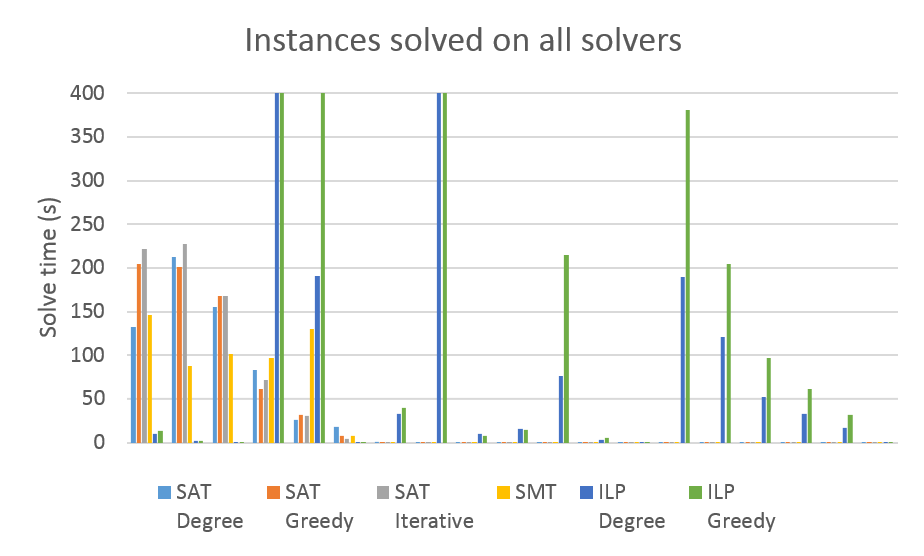
\includegraphics[width=0.5\textwidth]{figures/solve_time_comparison}
  \caption{Solve time per instance for instances solved with all approaches}
  \label{fig:solvetimecomparison}
\end{figure}

Table \ref{table:gccombinations} shows the total time needed to solve the instances which could be solved with all approaches.
It should be noted that while SMT looks faster than SAT, all SAT approaches are faster if instances which could not be solved on ILP are taken into account.
Figure \ref{fig:solvetimecomparison} shows the same solving time, but split up per instance.
It is interesting to see that while ILP solved more instances, it is generally much slower than SAT and SMT.

We then looked for a possible correlation between properties of the instance.
The solving time does not show any correlation with $N$, $M$, $N M$, $\frac{M}{N*(N-1)}$ (edge density) or $OPT$.
The best correlation we found can be seen in figure \ref{fig:nodecolorcombinations} and is the number of color combinations possible with optimal colors $N * OPT$.
The correlation is still weak at best, but for both SAT and ILP a general increase in solving time can be seen as it increases, which was not the case for the other metrics.
It can be seen that the solving time is much more influenced by it for SAT than for ILP, which is a possible explanation as to why ILP was able to solve a few of the larger instances.

\begin{figure}
  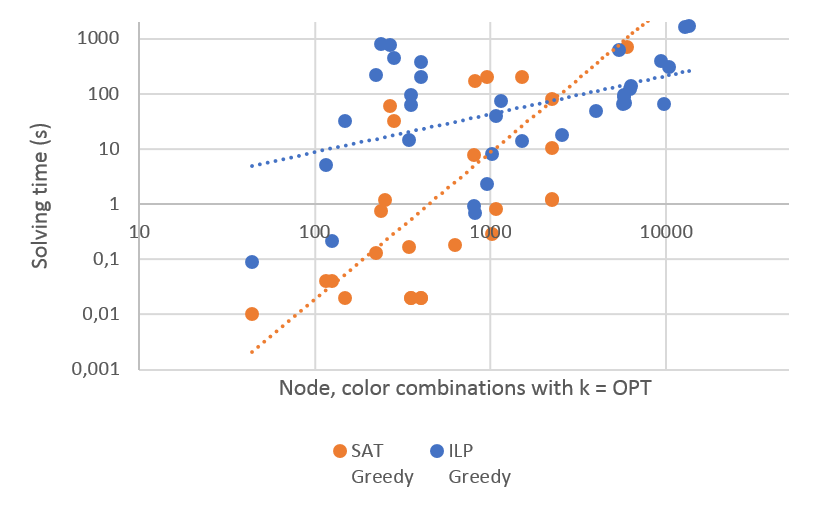
\includegraphics[width=0.5\textwidth]{figures/nodecolor_combinations_in_opt}
  \caption{Solve time plotted against possible node, color combinations $|N|*k$ with $k=OPT$}
  \label{fig:nodecolorcombinations}
\end{figure}

\section{Conclusion}

Our testing has not been as extensive as we initially had planned, primarily we can base our conclusion on only four distinct encodings while lots more are possible.

Our first result is that not all solver can be used to solve all problems.
While we know from theory that there is a polynomial transformation possible from every NP problem to every NP-Hard problem, that transformation is apparently not always known to the scientific community.
As such we can safely answer our research question with a no: not all solvers types can be used for all problems.

Our Graphs Coloring SAT, SMT and ILP comparison gives further insight into this question.
We shown that the specific approach makes relatively little difference and that the choise of solver type is much more important.
Specifically we've seen that for graph coloring ILP is able to solve a broader set of graph coloring instances and is less susceptible to increased problem size, but does perform worse on smaller instances than SAT and SMT do.

%TODO:Vertaling naar andere formalism: CSP (Constraint Satisfaction Problem), SAT, SMT, ILP en EA (Evolutionary Algorithms)
%TODO:RCPSP naar SAT is niet polynomiaal. We weten dat er één bestaat maar konden hem niet vinden.
In this paper, we managed to compare the performance of different types of solvers/algorithms such as SAT, SMT, ILP and greedy for the graph-coloring problem.
%With SAT solver we were able to find the minimum k for the graph-coloring problem by exploiting the upper/lower bounds using procedures for computing color k using greedy and binary search for guessing.
We couldn't find our way around with the RCPSP to SAT encoding. Even for small problem intances it was taking too long and there was also memory overflow. We know that such a polynomial formulation of the RCPSP as a SAT exist, but we couldn't find it.
\section{Discussion}

\section{Related and Future work}
\label{sec:relatedandfuture}
%TODO:Beschrijven wat andere mensen hebben gedaan en waarom dat relevant is.
In the literature there are some interesting previous work on solving graph coloring and resource constraint project scheduling problem. Here, we will discuss few of them and their methods that may have been relevant to our research.
Our work was based on earlier work done simmilar to, among others, \cite{ramani2004breaking}, where they optimally solve hard combinatorial problems (graph coloring as case study) by the reducing these to generic problems such as SAT and 0-1 ILP. They used a technique called symmetry breaking in an attempt to improve the performance of reduction-based methods, which are not competitive with problem-specific methods. This technique may be used together with the academic 0-1 solver PBS II to obtain bether performance results in future work.
%TODO:we hadden graag SMT en RCPSP getest.
Besides focusing on solving the graph coloring problem, we would have liked to expand our research on the RCPSP problem encoding to compare the performance of the ILP and SMT solvers.
%TODO:Wat SMT interessant maakt i.p.v. SAT is de 'Lazy clauses generation'.
%    :What makes SMT interesting to explore is the lazy clause generation.
%TODO:We hadden graag de truckjes in de paper van Horbach kunnen gebruiken
For the RCPSP problem there are a few papers that we found interesting. As in \cite{horbach2010boolean}, they adapted a satisfiability solver for there specific domain of the (RCPSP) problem. They were able to close several medium and large size benchmark instances from the PSLIB of the RCPSP that have never been closed before by providing tighter lower bounds and by finding bether feasible solutions. They cover the problem of dealing with linear inequalities over Boolean variable that can cause the number of clauses needed for the represention of many combinatorial problems to grow exponentially. We find this methods interesting enough to exploit further.
In \cite{klein1999computing} they used methonds and techniques for reducing problem data of RCPSP which can be exploited with the \emph{destructive improvement technique} that restricts a problem by setting a maximal objective function value F and try to contradict the feasibility of this reduced problem. This too might be interesting to evaluate the performance improvement. 
%TODO: However we couldn't get to solve the SAT encoding of RCPSP, due to...
We implemented an ILP encoding of the RCPSP problem to compare the solving time with the SAT encoding, 
but we didn't have the SAT solving times to compare with. 
It can be usefull to explore the SMT encoding of RCPSP, as it can work with among others integer, 
integer array and bitvector variables, and use its solving times and compare it with the ILP encoding.

%TODO: Deze referenties in de tekst verwerken of anders onzichtbaar opnemen in de 
\cite{alves2013resource}
\cite{abio2014encoding}
\cite{wu2013exploiting}
\cite{velev2009exploiting}
\cite{horbach2010boolean}
\cite{klein1999computing}
\cite{mingozzi1998exact}
\cite{sharma2011polynomial}
\cite{ramani2004breaking}
\cite{schutt2011explaining}
\cite{wille2008using}
\cite{malaguti2010survey}
\cite{cs395tGCtoSAT}

\bibliographystyle{plain}
\bibliography{in4336_report}



\appendix

\section*{}
\begin{table*}[b]
\caption{Solve time in seconds for all GC instances}
\label{table:resultsGCSolveTime}
\resizebox{\textwidth}{!}{%
\begin{tabular}{lllllllllllll}
\textbf{Instance} & \textbf{Type} & \textbf{N} & \textbf{M} & \textbf{OPT} & \textbf{Deg + 1} & \textbf{Greedy} & \textbf{\begin{tabular}[c]{@{}l@{}}SAT\\     Deg.\end{tabular}} & \textbf{\begin{tabular}[c]{@{}l@{}}SAT\\     Greedy\end{tabular}} & \textbf{\begin{tabular}[c]{@{}l@{}}SAT\\     It.\end{tabular}} & \textbf{SMT} & \textbf{\begin{tabular}[c]{@{}l@{}}ILP\\     Deg.\end{tabular}} & \textbf{\begin{tabular}[c]{@{}l@{}}ILP\\     Greedy\end{tabular}} \\
1-Insertions\_4 & CAR & 67 & 232 & 4 & 23 & 5 & 83,72 & 61,05 & 71,57 & 96,56 & 751,44 & 751,44 \\
2-Insertions\_3 & CAR & 37 & 72 & 4 & 10 & 4 & 0,05 & 0,02 & 0,03 & 0,03 & 16,34 & 31,47 \\
2-Insertions\_4 & CAR & 149 & 541 & 4 & 38 & 5 &  &  &  &  &  &  \\
3-Insertions\_3 & CAR & 56 & 110 & 4 & 12 & 4 & 0,18 & 0,13 & 0,15 & 0,11 & 76,67 & 215,06 \\
3-Insertions\_4 & CAR & 281 & 1046 &  & 57 & 5 &  &  &  &  &  &  \\
4-Insertions\_3 & CAR & 79 & 156 & 3 & 14 & 4 & 0,77 & 0,76 & 0,88 & 0,45 & 732,79 & 789,4 \\
4-Insertions\_4 & CAR & 475 & 1795 &  & 80 & 5 &  &  &  &  &  &  \\
DSJC125.1 & DSJ & 125 & 736 & 5 & 24 & 8 & 0,23 & 0,18 & 0,18 & 0,15 &  &  \\
DSJC125.5 & DSJ & 125 & 3891 &  & 76 & 26 &  &  &  &  &  &  \\
DSJC125.9 & DSJ & 125 & 6961 &  & 121 & 56 &  &  &  &  &  &  \\
DSJR500.1 & DSJ & 500 & 3555 & 12 & 26 & 15 &  & 716,01 & 951,31 &  &  &  \\
qg.order30 & GOM & 900 & 26100 & 30 & 59 & 32 &  &  &  &  &  &  \\
qg.order40 & GOM & 1600 & 62400 & 40 & 79 & 64 &  &  &  &  &  &  \\
qg.order60 & GOM & 3600 & 212400 & 60 & 119 & 64 &  &  &  &  &  &  \\
qg.order100 & GOM & 10000 & 990000 & 100 & 199 & 128 &  &  &  &  &  &  \\
le450\_5a & LEI & 450 & 5714 & 5 & 43 & 14 & 9,98 & 10,49 & 0,56 & 25,69 &  &  \\
le450\_5b & LEI & 450 & 5734 & 5 & 43 & 13 & 29,54 & 78,76 & 1,29 & 270,02 &  &  \\
le450\_5c & LEI & 450 & 9803 & 5 & 67 & 17 & 3,74 & 1,18 & 0,82 & 4,75 &  &  \\
le450\_5d & LEI & 450 & 9757 & 5 & 69 & 18 & 9 & 1,22 & 0,79 & 5,02 &  &  \\
le450\_15a & LEI & 450 & 8168 & 15 & 100 & 22 &  &  &  &  &  &  \\
le450\_15b & LEI & 450 & 8169 & 15 & 95 & 22 &  &  &  &  &  &  \\
le450\_15c & LEI & 450 & 16680 & 15 & 140 & 30 &  &  &  &  &  &  \\
le450\_15d & LEI & 450 & 16750 & 15 & 139 & 31 &  &  &  &  &  &  \\
le450\_25a & LEI & 450 & 8260 & 25 & 129 & 28 &  &  &  &  &  &  \\
le450\_25b & LEI & 450 & 8263 & 25 & 112 & 27 &  &  &  &  &  &  \\
le450\_25c & LEI & 450 & 17343 & 25 & 180 & 37 &  &  &  &  &  &  \\
le450\_25d & LEI & 450 & 17425 & 25 & 158 & 35 &  &  &  &  &  &  \\
mug100\_1 & MIZ & 100 & 166 & 4 & 5 & 4 & 0,03 & 0,02 & 0,04 & 0,03 & 121,41 & 204,57 \\
mug100\_25 & MIZ & 100 & 166 & 4 & 5 & 4 & 0,03 & 0,02 & 0,04 & 0,03 & 189,6 & 381,3 \\
mug88\_1 & MIZ & 88 & 146 & 4 & 5 & 4 & 0,03 & 0,02 & 0,03 & 0,03 & 33,16 & 61,55 \\
mug88\_25 & MIZ & 88 & 146 & 4 & 5 & 4 & 0,03 & 0,02 & 0,03 & 0,03 & 51,95 & 96,52 \\
myciel3 & MYC & 11 & 20 & 4 & 6 & 4 & 0,02 & 0,01 & 0,01 & 0,02 & 0,13 & 0,09 \\
myciel4 & MYC & 23 & 71 & 5 & 12 & 5 & 0,06 & 0,04 & 0,05 & 0,05 & 3,52 & 5,05 \\
myciel5 & MYC & 47 & 236 & 6 & 24 & 6 & 26,34 & 31,39 & 31,06 & 130,04 & 190,64 & 452,03 \\
myciel6 & MYC & 95 & 755 & 7 & 48 & 7 &  &  &  &  &  &  \\
myciel7 & MYC & 191 & 2360 & 8 & 96 & 8 &  &  &  &  &  &  \\
fpsol2.i.1 & REG & 496 & 11654 & 65 & 253 & 65 &  &  &  &  &  &  \\
fpsol2.i.2 & REG & 451 & 8691 & 30 & 347 & 30 &  &  &  &  & 1607,03 & 1661,68 \\
fpsol2.i.3 & REG & 425 & 8688 & 30 & 347 & 30 &  &  &  &  & 1390,73 & 1639,06 \\
inithx.i.1 & REG & 864 & 18707 & 54 & 503 & 54 &  &  &  &  &  &  \\
inithx.i.2 & REG & 645 & 13979 & 31 & 542 & 31 &  &  &  &  &  &  \\
inithx.i.3 & REG & 621 & 13969 & 31 & 543 & 31 &  &  &  &  &  &  \\
mulsol.i.1 & REG & 197 & 3925 & 49 & 122 & 49 &  &  &  &  & 52,14 & 65,53 \\
mulsol.i.2 & REG & 188 & 3885 & 31 & 157 & 31 &  &  &  &  & 59,02 & 66,69 \\
mulsol.i.3 & REG & 184 & 3916 & 31 & 158 & 31 &  &  &  &  & 61,67 & 65,3 \\
mulsol.i.4 & REG & 185 & 3946 & 31 & 159 & 31 &  &  &  &  & 68,68 & 94,96 \\
mulsol.i.5 & REG & 186 & 3973 & 31 & 160 & 31 &  &  &  &  & 71,37 & 87,64 \\
zeroin.i.1 & REG & 211 & 4100 & 49 & 112 & 49 &  &  &  &  & 246,82 & 299,98 \\
zeroin.i.2 & REG & 211 & 3541 & 30 & 141 & 30 &  &  &  &  & 93,04 & 135,51 \\
zeroin.i.3 & REG & 206 & 3540 & 30 & 141 & 30 &  &  &  &  & 75,35 & 119,95 \\
anna & SGB-B & 138 & 986 & 11 & 72 & 12 & 131,92 & 204,31 & 221,23 & 145,58 & 10,41 & 13,62 \\
david & SGB-B & 87 & 812 & 11 & 83 & 12 & 212,89 & 200,58 & 226,91 & 87,51 & 2,04 & 2,28 \\
huck & SGB-B & 74 & 602 & 11 & 54 & 11 & 155,58 & 167,33 & 167,67 & 101,16 & 0,66 & 0,7 \\
jean & SGB-B & 80 & 508 & 10 & 37 & 10 & 18,33 & 7,61 & 4,48 & 7,28 & 0,9 & 0,91 \\
games120 & SGB-G & 120 & 1276 & 9 & 14 & 9 & 1,18 & 0,82 & 0,98 & 1,06 & 32,52 & 39,14 \\
miles250 & SGB-S & 128 & 774 & 8 & 17 & 9 & 0,6 & 0,29 & 0,38 & 0,29 & 10,11 & 8,16 \\
miles500 & SGB-S & 128 & 2340 & 20 & 39 & 22 &  &  &  &  & 18,16 & 18 \\
miles750 & SGB-S & 128 & 4226 & 31 & 65 & 34 &  &  &  &  & 40,76 & 49,02 \\
miles1000 & SGB-S & 128 & 6432 & 42 & 87 & 44 &  &  &  &  & 749,51 & 615,09 \\
miles1500 & SGB-S & 128 & 10396 & 73 & 107 & 76 &  &  &  &  & 212,36 & 397,84 \\
queen5\_5 & SGB-Q & 25 & 320 & 5 & 17 & 8 & 0,09 & 0,04 & 0,03 & 0,07 & 0,28 & 0,21 \\
queen6\_6 & SGB-Q & 36 & 580 & 7 & 20 & 11 & 1,33 & 1,19 & 1,15 & 1,45 &  &  \\
queen7\_7 & SGB-Q & 49 & 952 & 7 & 25 & 10 & 0,27 & 0,17 & 0,15 & 0,31 & 15,2 & 14,28 \\
queen8\_12 & SGB-Q & 96 & 2736 & 12 & 33 & 15 &  &  &  &  & 79,55 & 74,84 \\
queen8\_8 & SGB-Q & 64 & 1456 & 9 & 28 & 13 &  &  &  &  &  &  \\
queen9\_9 & SGB-Q & 81 & 2112 & 10 & 33 & 16 &  &  &  &  &  & 
\end{tabular}
}
\end{table*}

\section*{}
\begin{table}
\caption{Graph coloring instance types}
\label{my-label}
\begin{tabular}{ll}
\textbf{Type} & \textbf{Description} \\
\textbf{CAR}   & Based on MYC graphs with added nodes with identical density                                                    \\
\textbf{DSJ}   & Random graphs made by Johnson et al. {[}13{]}.                                                                 \\
\textbf{GOM}   & Latin squares                                                                                                  \\
\textbf{LEI}   & Leighton Graphs, these have specic kinds of asymmetry                                                          \\
\textbf{MIZ}   & No information was available about this type                                                                   \\
\textbf{MYC}   & Graphs made from Mycielski transformations, which ensures graphs without triangles                             \\
\textbf{REG}   & Graphs made from register allocation instances from specic programs                                           \\
\textbf{SGB-B} & Graphs based on character interactions within books                                                            \\
\textbf{SGB-G} & Graphs based on footballs teams playing against each other                                                     \\
\textbf{SGB-M} & Geometric graphs of cities connected if they are close enough                                                  \\
\textbf{SGB-Q} & Queen graphs, giving the number of queens that can be placed on an NxN graph without them attacking each other
\end{tabular}
\end{table}

\section*{}


\end{document}